\section{Experiments}
\label{sec:experiments}

\subsection{Setup}
\label{sec:setup}

\noindent\textbf{Models.}
The main target is \qwenS~\cite{bai2025qwen25vl} with the released \vispec draft model for it.
On \qwenL we compare the released \vispec and \hivis draft models for that target.
A separate set of runs pairs \llava with Vicuna 7B~\cite{liu2024llavanext} and its \vispec draft model.

\noindent\textbf{Single images.}
The Qwen models answer 100 TextVQA questions~\cite{singh2019textvqa}, drawn by a seeded shuffle of the validation set, and caption 100 images of the COCO Karpathy test split~\cite{chen2015coco,karpathy2015deep}.
Each benchmark runs in two answer styles.
The long style asks for a detailed explanation or description and measures speed, because its answers run to hundreds of tokens.
The short style asks for a single word or phrase, or a one-sentence caption, and measures quality with VQA accuracy and CIDEr-D~\cite{vedantam2015cider}.
The \llava runs answer TextVQA, GQA~\cite{hudson2019gqa} and MM-Vet~\cite{yu2024mmvet} in the long style and TextVQA and GQA in the short style.

\noindent\textbf{Manga page windows.}
\rvp extends Re:Verse~\cite{baranwal2025reverse} with a narration of the story aligned to every manga page.
We split volume~1 into \pagesN windows of five or six consecutive pages, give each window to the model as images only, and ask it to summarize the story in order.
The prompts hold \pagesPromptMin to \pagesPromptMax tokens, a mean of \pagesPromptMean, of which \pagesImageShare\% are image tokens, against \promptTextvqa for a TextVQA prompt.
We score each summary against the narration of its pages with ROUGE-1~\cite{lin2004rouge} and BERTScore~\cite{zhang2020bertscore} F1.
The pages are credited to Yen Press, their English publisher, and are used for non-commercial research only.

\noindent\looseness=-1\textbf{Decoding and timing.} 
All runs decode greedily in bf16 at batch size one with at most 1,024 new tokens, and the draft tree has depth 3, eight candidates per node and 30 tokens in total.
Each Qwen job runs on one NVIDIA RTX A6000 with 48\,GB and runs AR and the speculative decoders in sequence, and every speedup divides the mean AR latency by the mean latency of the speculative decoder in the same job.
Repeated jobs with identical outputs give the spread between jobs, which we report as a range.
The \llava runs were made on separate hardware with the same decoding settings \TODO{confirm the GPU of the LLaVA runs}.

\subsection{Speedup and output exactness}
\label{sec:exactness}

\begin{table*}[t]
\centering
\footnotesize
\setlength{\tabcolsep}{4.2pt}
\begin{tabular}{lllccccccc}
\toprule
& & & \multicolumn{3}{c}{Long answers} & \multicolumn{4}{c}{Short answers} \\
\cmidrule(lr){4-6}\cmidrule(lr){7-10}
Target & Drafter & Benchmark & Speedup & $\tau$ & Same as AR & Speedup & Quality, AR & Quality, drafter & Same as AR \\
\midrule
\multirow{3}{*}{\llava} & \multirow{3}{*}{\vispec} & TextVQA & \llavaLongTextvqaSpeedup & \llavaLongTextvqaAccept & \llavaLongTextvqaSame/\llavaLongTextvqaTotal & \llavaShortTextvqaSpeedup & \llavaShortTextvqaAcc & \llavaShortTextvqaAcc & \llavaShortTextvqaSame/100 \\
 & & GQA & \llavaLongGqaSpeedup & \llavaLongGqaAccept & \llavaLongGqaSame/\llavaLongGqaTotal & \llavaShortGqaSpeedup & \llavaShortGqaAcc & \llavaShortGqaAcc & \llavaShortGqaSame/100 \\
 & & MM-Vet & \llavaLongMmvetSpeedup & \llavaLongMmvetAccept & \llavaLongMmvetSame/\llavaLongMmvetTotal & n/a & n/a & n/a & n/a \\
\midrule
\multirow{2}{*}{\qwenS} & \multirow{2}{*}{\vispec} & TextVQA & \tbLongTextvqaSpeedMin to \tbLongTextvqaSpeedMax & \tbLongTextvqaAccept & \tbLongTextvqaSame/\tbLongTextvqaTotal & \tbShortTextvqaSpeedMin & \tbShortTextvqaQualAr & \tbShortTextvqaQualSpec & \tbShortTextvqaSame/\tbShortTextvqaTotal \\
 & & COCO & \tbLongCocoSpeedMin to \tbLongCocoSpeedMax & \tbLongCocoAccept & \tbLongCocoSame/\tbLongCocoTotal & \tbShortCocoSpeedMin & \tbShortCocoQualAr & \tbShortCocoQualSpec & \tbShortCocoSame/\tbShortCocoTotal \\
\midrule
\multirow{4}{*}{\qwenL} & \multirow{2}{*}{\vispec} & TextVQA & \sbLongTextvqaVisSpeedMin to \sbLongTextvqaVisSpeedMax & \sbLongTextvqaVisAccept & \sbLongTextvqaVisSame/100 & \sbShortTextvqaVisSpeedMin & \sbShortTextvqaQualAr & \sbShortTextvqaVisQual & \sbShortTextvqaVisSame/100 \\
 & & COCO & \sbLongCocoVisSpeedMin to \sbLongCocoVisSpeedMax & \sbLongCocoVisAccept & \sbLongCocoVisSame/100 & \sbShortCocoVisSpeedMin & \sbShortCocoQualAr & \sbShortCocoVisQual & \sbShortCocoVisSame/100 \\
\cmidrule{2-10}
 & \multirow{2}{*}{\hivis} & TextVQA & \sbLongTextvqaHivSpeedMin to \sbLongTextvqaHivSpeedMax & \sbLongTextvqaHivAccept & \sbLongTextvqaHivSame/100 & \sbShortTextvqaHivSpeedMin & \sbShortTextvqaQualAr & \sbShortTextvqaHivQual & \sbShortTextvqaHivSame/100 \\
 & & COCO & \sbLongCocoHivSpeedMin to \sbLongCocoHivSpeedMax & \sbLongCocoHivAccept & \sbLongCocoHivSame/100 & \sbShortCocoHivSpeedMin & \sbShortCocoQualAr & \sbShortCocoHivQual & \sbShortCocoHivSame/100 \\
\bottomrule
\end{tabular}
\caption{\textbf{Speculative decoding on single images.} Speedup is the mean AR latency over the mean latency of the drafter in the same job, given as the range over three jobs for long answers on the Qwen targets and from one job otherwise. $\tau$ is the mean number of accepted draft tokens per decoding step, and Same as AR counts outputs whose tokens equal those of AR. Quality is VQA accuracy for TextVQA, exact match for GQA and CIDEr-D for COCO captions. Long answers are not scored, because the strict scorers reject paragraph answers. The \llava rows come from a separate set of runs with the same decoding settings.}
\label{tab:main}
\end{table*}


\noindent\looseness=-1\textbf{Long answers.} 
Across all three targets the speculative decoders run long answers at about twice the speed of AR (\cref{tab:main}).
On \qwenS, \vispec is \tbLongTextvqaSpeedMin to \tbLongTextvqaSpeedMax times faster than AR on long TextVQA answers and \tbLongCocoSpeedMin to \tbLongCocoSpeedMax times on long captions, with \tbLongTextvqaAccept and \tbLongCocoAccept accepted draft tokens per step.
On \qwenL the two drafters reach \sbLongTextvqaVisSpeedMin to \sbLongCocoHivSpeedMax times, and on \llava \vispec reaches \llavaLongGqaSpeedup to \llavaLongTextvqaSpeedup times across its three benchmarks.

\noindent\textbf{Short answers.}
A short answer gains nothing.
On short TextVQA answers \vispec runs at \tbShortTextvqaSpeedMin times the speed of AR on \qwenS, because the time to the first token is \tbShortTextvqaShare\% of its latency, and the same holds for \hivis on \qwenL and for \llava, where the first token takes \llavaShortFirstShareMin to \llavaShortFirstShareMax\% of the time.
Short captions are long enough to gain \tbShortCocoSpeedMin times on \qwenS.

\begin{figure}[t]
\centering
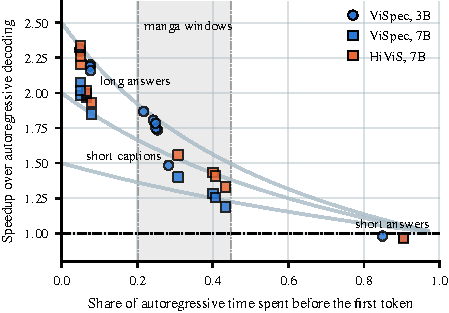
\includegraphics{figures/amdahl.pdf}
\caption{\textbf{Speedup against the share of time before the first token.} Each point is one benchmark and answer style in one job. The grey curves give \cref{eq:amdahl} for a decoding speedup of 1.5, 2 and 2.5, the values at which they meet the vertical axis, and the shaded band holds the manga windows of both targets.}
\label{fig:amdahl}
\end{figure}

\noindent\textbf{One law for every setting.}
\Cref{fig:amdahl} places every Qwen setting by the share of AR time spent before the first token.
The points follow \cref{eq:amdahl}, with decoding speedups between about 1.5 and 2.5, and their horizontal position, not the drafter, sets how much of that decoding gain survives end to end.
Long answers spend under a tenth of their AR time before the first token, short captions close to a third and short TextVQA answers nearly all of it.

\begin{figure}[t]
\centering
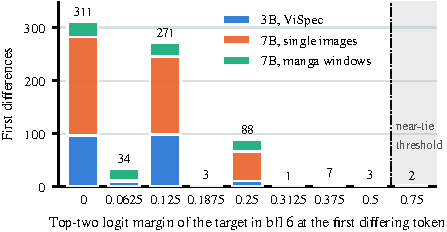
\includegraphics{figures/margins.pdf}
\caption{\textbf{Margin of the target's top two logits at every first difference from AR.} The counts cover every diagnosed output of \vispec on \qwenS and of both drafters on \qwenL, and the shaded region lies beyond the near-tie threshold.}
\label{fig:margins}
\end{figure}

\noindent\textbf{Exactness.}
In full precision every speculative decoder reproduces AR token for token, in \fpeAll of \fpqAll replayed samples across both Qwen targets, three eviction settings and the manga windows.
In bf16 the outputs often differ, on long answers more than on short ones, because a change at one token sends the rest of a long answer along a different path.
The divergence diagnosis finds the cause at the first differing token (\cref{fig:margins}).
Of \diagCasesAll first differences, \diagNearAll are near-ties with a bf16 margin of at most 0.5 logits and a median of \diagNearMedian.
The remaining \diagOtherAll are one token of one manga window that \vispec and \hivis on \qwenL both choose over AR's token.
Its bf16 margin is \diagBigBf, and in full precision the margin falls to \diagBigFp in favour of AR's token, so it is a near-tie in full precision.
Short-answer quality confirms that these changes do not degrade the answers, with VQA accuracy and CIDEr-D within one to two points of AR and identical scores on \qwenL TextVQA.

\subsection{Visual input during decoding}
\label{sec:visual}

\noindent\looseness=-1\textbf{A draft model without the image.} 
On \qwenL, \hivis is at least as fast as \vispec although its draft model never sees an image token.
It runs \sbLongCocoHovMin to \sbLongCocoHovMax times faster than \vispec on long captions, and \sbLongTextvqaHovMin to \sbLongTextvqaHovMax times on long TextVQA answers, which is within the spread between jobs.
On long captions it accepts \sbLongCocoHivAccept draft tokens per step against \sbLongCocoVisAccept at nearly the same step time, \sbCocoHivStep against \sbCocoVisStep\,ms, so each output token costs \sbCocoHivTpot instead of \sbCocoVisTpot\,ms.
The target's hidden states can therefore carry what the draft model needs from the image.
The two draft models are separately trained checkpoints, so the comparison covers each drafter as a whole and not its visual input alone.

\begin{figure*}[t]
\centering
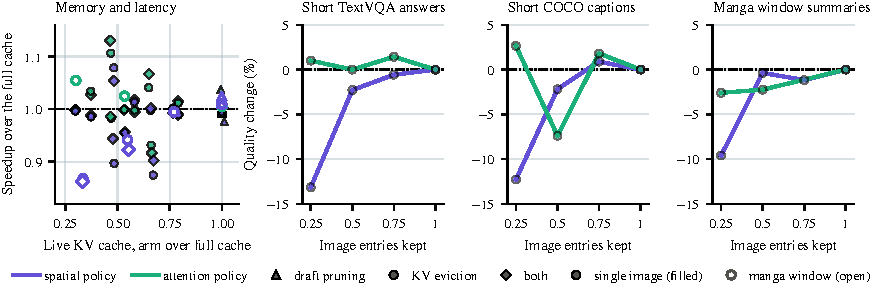
\includegraphics{figures/sparsity.pdf}
\caption{\textbf{Visual sparsity in \vispec on \qwenS.} The left panel places every arm below full retention by its live KV cache and its speedup, both relative to the same policy at full retention for single images and to the full cache of the same job for manga windows. The other panels give the change in quality under KV eviction as the share of image entries kept falls, in VQA accuracy, CIDEr-D and ROUGE-1.}
\label{fig:sparsity}
\end{figure*}


\noindent\looseness=-1\textbf{Draft pruning.} 
Pruning what the \vispec adaptor reads leaves decoding as it was (\cref{fig:sparsity}).
Acceptance moves by \spDraftAccMin to +\spDraftAccMax tokens per step and latency by a factor of \spDraftLatMin to \spDraftLatMax against the full input, and the cache does not change.
The adaptor already reduces each image to two queries, so pruning removes tokens the draft model never attends to at any decoding step.

\noindent\textbf{KV eviction.}
Eviction shrinks the live KV cache to \spEvictKvMin to \spEvictKvMax of the full cache without changing the time to the first token, whose ratio stays between \spEvictTtftMin and \spEvictTtftMax.
End-to-end latency ranges from \spEvictLatMin to \spEvictLatMax times that of the full cache, and these ratios follow the length of the outputs and a rise in acceptance under eviction, to \spLongTextvqaAccMin to \spLongTextvqaAccMax tokens per step on long TextVQA answers.
The spatial policy at a quarter of the image entries costs \spShortTextvqaRef to \spShortTextvqaSpatialQuarter in VQA accuracy and \spShortCocoRef to \spShortCocoSpatialQuarter in CIDEr-D, while the attention policy at the same budget scores \spShortTextvqaAttentionQuarter and \spShortCocoAttentionQuarter.
On long answers every eviction arm changes almost every output, with \spLongSameMin to \spLongSameMax of 100 identical to the full cache.
Applying both forms together tracks eviction alone.

\begin{figure}[t]
\centering
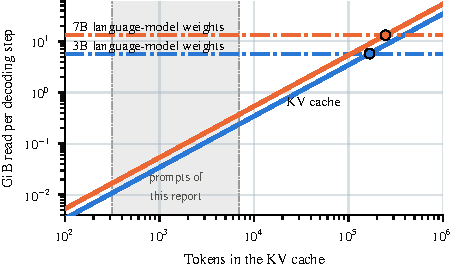
\includegraphics{figures/cost.pdf}
\caption{\textbf{Bytes read by one decoding step at batch size one} under \cref{eq:bytes}. Dash-dotted lines give the language-model weights and solid lines the KV cache, and a dot marks the length at which the two are equal. The shaded band spans the shortest to the longest prompt of this report, a COCO prompt to a manga window.}
\label{fig:cost}
\end{figure}

\noindent\textbf{Memory traffic of a decoding step.}
\Cref{eq:bytes} explains why neither form moves the cost of a step (\cref{fig:cost}).
\qwenS stores \costTbKvPerToken bytes of cache per token and reads \costTbWeights\,GiB of language-model weights at every step, so the whole cache is \costTbThousand\% of the bytes of a step at a thousand tokens and \costTbSevenThousand\% at seven thousand, and the two become equal only near \costTbEqual tokens.
For \qwenL the figures are \costSbKvPerToken bytes, \costSbWeights\,GiB and \costSbEqual tokens.
Evicting every image entry would thus remove only a small fraction of the memory traffic of a step.
A decode profile adds that the GPU executes kernels for only \profileBusyMin to \profileBusyMax\% of an unprofiled step and waits on the host for the rest, so cheaper kernels would barely shorten the step either.
At batch size one visual sparsity therefore trades output agreement, and at low budgets quality, for memory.

\subsection{Manga page windows}
\label{sec:pages}

\begin{table*}[t]
\centering
\footnotesize
\setlength{\tabcolsep}{4.5pt}
\begin{tabular}{llcccccccc}
\toprule
Target & Drafter & Jobs & Speedup & Decoding speedup & TTFT share & $\tau$ & Output tokens & Windows at the limit & ROUGE-1 \\
 & & & & below the limit & of the drafter & & AR, drafter & AR, drafter & AR, drafter \\
\midrule
\qwenS & \vispec & \pagesJobs & \tbPagesSpeedMin to \tbPagesSpeedMax & \tbPagesDecodeMin to \tbPagesDecodeMax & \tbPagesShareMin to \tbPagesShareMax\% & \tbPagesAccept & \tbPagesLenAr, \tbPagesLenSpec & \tbPagesCapAr, \tbPagesCapSpec & \tbPagesQualAr, \tbPagesQualSpec \\
\midrule
\multirow{2}{*}{\qwenL} & \vispec & \sbPagesJobs & \sbPagesVisSpeedMin to \sbPagesVisSpeedMax & \sbPagesVisDecodeMin to \sbPagesVisDecodeMax & \sbPagesVisShare\% & \sbPagesVisAccept & \sbPagesArLen, \sbPagesVisLen & \sbPagesArCap, \sbPagesVisCap & \sbPagesArRouge, \sbPagesVisRouge \\
 & \hivis & \sbPagesJobs & \sbPagesHivSpeedMin to \sbPagesHivSpeedMax & \sbPagesHivDecodeMin to \sbPagesHivDecodeMax & \sbPagesHivShare\% & \sbPagesHivAccept & \sbPagesArLen, \sbPagesHivLen & \sbPagesArCap, \sbPagesHivCap & \sbPagesArRouge, \sbPagesHivRouge \\
\bottomrule
\end{tabular}
\caption{\textbf{Speculative decoding on manga page windows.} Each window holds five or six pages of \rvp, and each job runs all \pagesN windows with identical outputs for each method across jobs. The decoding speedup divides the decoding time of AR by that of the drafter over the windows where neither reaches the limit of 1,024 new tokens, \tbPagesDecodeN windows for \vispec on \qwenS and \sbPagesVisDecodeN and \sbPagesHivDecodeN for \vispec and \hivis on \qwenL. The TTFT share is the time to the first token over the latency of the drafter.}
\label{tab:pages}
\end{table*}


\noindent\looseness=-1\textbf{The first token caps the gain.} 
On five- and six-page windows \vispec is \tbPagesSpeedMin to \tbPagesSpeedMax times faster than AR on \qwenS over \pagesJobs jobs with identical outputs, against more than two times on long single-image answers (\cref{tab:pages}).
Prompt processing takes \tbPagesTtftMin to \tbPagesTtftMax\,s per window, \tbPagesShareMin to \tbPagesShareMax\% of the speculative decoder's time, and by \cref{eq:amdahl} it bounds the speedup at \tbPagesBoundMin to \tbPagesBoundMax times even for infinitely fast decoding.
The decoding phase itself gains \tbPagesDecodeMin to \tbPagesDecodeMax times over the \tbPagesDecodeN windows where neither method reaches the token limit, against \tbSingleDecodeMin to \tbSingleDecodeMax times on long single-image answers, matching its lower acceptance of \tbPagesAccept.

\noindent\looseness=-1\textbf{The larger model.} 
On \qwenL the cap tightens.
The time to the first token is \sbPagesTtftMin to \sbPagesTtftMax\,s for all three methods, \sbPagesVisShare\% of the time of \vispec and \sbPagesHivShare\% of that of \hivis, and the AR summaries are shorter than on \qwenS, \sbPagesArLen against \tbPagesLenAr tokens, which leaves less decoding to accelerate.
\vispec is \sbPagesVisSpeedMin to \sbPagesVisSpeedMax and \hivis \sbPagesHivSpeedMin to \sbPagesHivSpeedMax times faster than AR (\cref{fig:teaser}).

\noindent\textbf{A drafter without the pages.}
\hivis leads \vispec by \sbPagesHovMin times in every job, and it accepts \sbPagesHivAccept draft tokens per step against \sbPagesVisAccept although its draft model receives identical text for every window.
Over the \sbPagesHovDecodeN windows where neither drafter reaches the token limit, \hivis decodes \sbPagesHovDecodeMin times faster, and the rest of its lead comes from shorter summaries, \sbPagesHivLen against \sbPagesVisLen tokens.
Summary quality stays close to AR for both drafters on both targets.

\noindent\looseness=-1\textbf{Visual sparsity on pages.} 
On the windows the full cache of \qwenS holds \spPagesKvFull\,MiB, and evicting three quarters of the image entries leaves \spPagesKvQuarterAttention\,MiB with the attention policy and \spPagesKvQuarterSpatial\,MiB with the spatial policy.
The attention policy at that budget is \spPagesLatQuarterAttention times as fast as the full cache with a ROUGE-1 of \spPagesRougeQuarterAttention against \spPagesRougeRef.
The spatial policy drives the summaries into loops, lowering the share of distinct token 4-grams from \spPagesDistinctRef to \spPagesDistinctQuarterSpatial and sending \spPagesCapQuarterSpatial windows to the token limit against \spPagesCapRef, so it runs at \spPagesLatQuarterSpatial times the speed of the full cache with a ROUGE-1 of \spPagesRougeQuarterSpatial.
